\documentclass{standalone}
\usepackage{tikz}
\usetikzlibrary{shapes.geometric, arrows}

\begin{document}

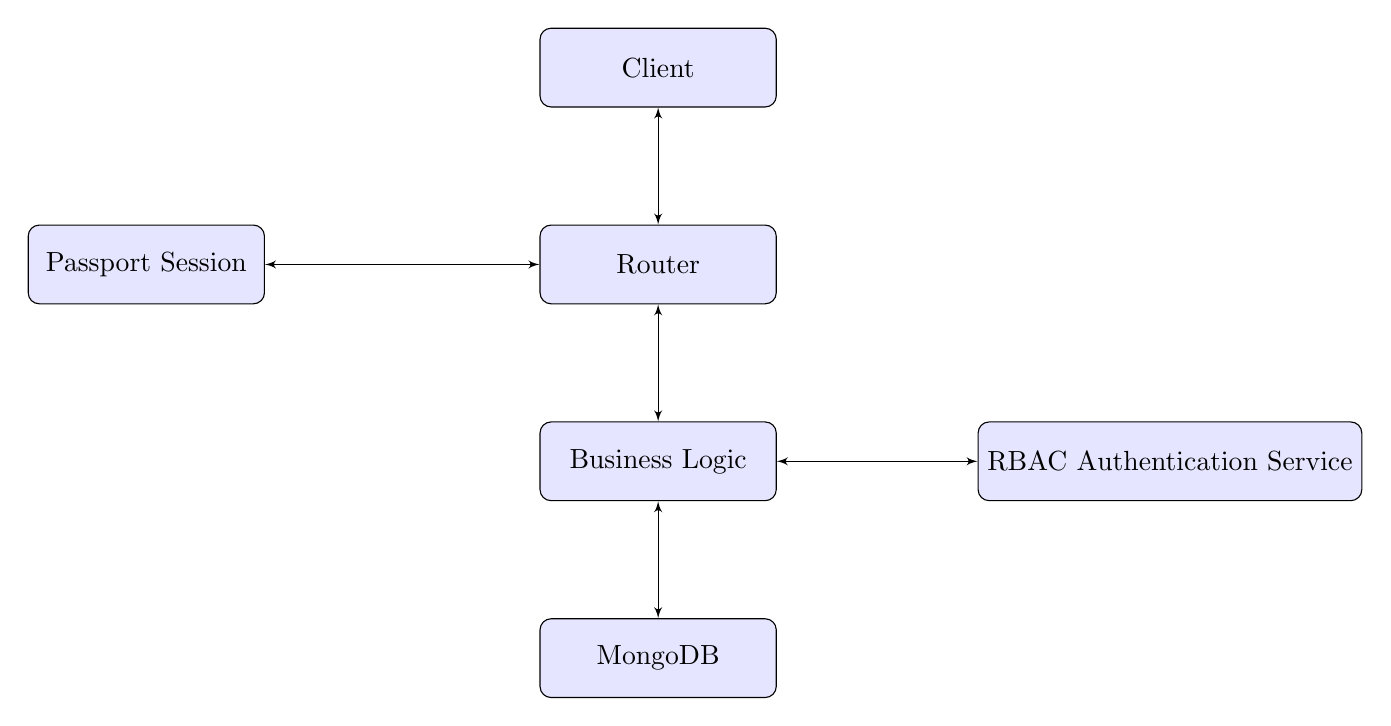
\begin{tikzpicture}[node distance=2.5cm, >=latex']

% Stili dei blocchi
\tikzstyle{block} = [rectangle, draw, fill=blue!10,
    minimum width=3cm, minimum height=1cm, text centered, rounded corners]
\tikzstyle{arrow} = [thick,->,>=stealth]

% Nodi
\node (client) [block] {Client};
\node (router) [block, below of=client] {Router};
\node (passport) [block, left of=router, xshift=-4cm] { Passport Session };
\node (logic) [block, below of=router] {Business Logic};
\node (auth) [block, right of=logic, xshift=4cm] {RBAC Authentication Service};
\node (db) [block, below of=logic] {MongoDB};

% Frecce
\draw [<->] (client) -- (router);
\draw [<->] (router) -- (passport);
\draw [<->] (router) -- (logic);
\draw [<->] (logic) -- (db);
\draw [<->] (logic) -- (auth);

\end{tikzpicture}

\end{document}
